\documentclass{tikzposter} %Options for format can be included here
\usepackage{pgfplots}
\usepackage{amsmath}
\usepackage{amsfonts}
\usepackage{amssymb}

\renewcommand\Re{\mathop{\rm Re}\nolimits}
\renewcommand\Im{\mathop{\rm Im}\nolimits}

 % Title, Author, Institute
\title{
\vbox{
Inverse problems for Sturm-Liouville operators  
with Bessel-type singularity inside an interval
}
}
\author{Alexey Fedoseev}
\institute{Saratov State University, Russia}
%\titlegraphic{LogoGraphic Inserted Here}

 %Choose Layout
\usetheme{Default}

\begin{document}

 % Title block with title, author, logo, etc.
\maketitle

 \block{What is Inverse Problems?}
{
Solution of an inverse problem entails determining unknown causes, based on observation of their effects.

Inverse problem: causes -> consequences (observations, effects, results)

Direct problem: consequences -> causes
}

\block{First Result in Spectral Inverse Problems Theory}{
The field of inverse problems was first discovered and introduced by Soviet-Armenian physicist, Viktor Ambartsumian.

While still a student, Ambartsumian thoroughly studied the theory of atomic structure, the formation of energy levels, and the Schrödinger equation and its properties, and when he mastered the theory of eigenvalues of differential equations, he pointed out the apparent analogy between discrete energy levels and the eigenvalues of differential equations. He then asked: given a family of eigenvalues, is it possible to find the form of the equations whose eigenvalues they are? Essentially Ambartsumian was examining the inverse Sturm–Liouville problem, which dealt with determining the equations of a vibrating string. This paper was published in 1929 in the German physics journal Zeitschrift für Physik and remained in obscurity for a rather long time. Describing this situation after many decades, Ambartsumian said, "If an astronomer publishes an article with a mathematical content in a physics journal, then the most likely thing that will happen to it is oblivion."

Nonetheless, toward the end of the Second World War, this article, written by the 20-year-old Ambartsumian, was found by Swedish mathematicians and formed the starting point for a whole area of research on inverse problems, becoming the foundation of an entire discipline.
}

\block{}{

\begin{tikzfigure}[A figure can be made withoes not work]
\includegraphics[scale=1]{Neptune.pdf}
\includegraphics[scale=1]{spectra.pdf}
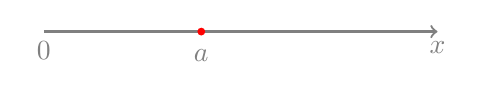
\begin{tikzpicture}[scale=1]
\draw [->, color=gray,thick] (0,0) node[below] {$0$}-- (5,0) node[below] {$x$};
\node[shape=circle,fill=red,scale=0.3] at (2,0) {};
\node[below,color=gray] at (2,-0.1) {$a$};
\end{tikzpicture}
\end{tikzfigure}
}

\block{Object}{
Consider the differential equation
\begin{equation}
\ell y = -y''+\Big(\frac{\nu_0}{(x-a)^2}+q(x)\Big)y=\lambda y,\quad x>0,
\label{initeq}
\end{equation}
on the half-line with a Bessel-type singularity at an interior point $a>0$. Here $q(x)$ is a complex-valued function and $\nu_0$ is a complex number. Let $\nu_0=\nu^2-1/4$ and to be definite, we assume that  $Re\,\nu>0,$ $\nu\neq 1,2,\ldots$ (the other cases require minor modifications). We also assume that $q(x)|x-~a|^{\min(0,1-2Re\,\nu)} \in L(0,T)$ for some $T>a$ and $q(x)\in L(T,\infty)$. We denote the class of such functions $q(x)$ by $W$.

CHANGE THIS!!!!!!!!!!

The paper deals with the boundary value problem  ${\cal L=L}(q)$ for differential equation \eqref{initeq} with the Dirichlet boundary condition $y(0)=0$ and an additional \textit{matching conditions} near the singular point $x=a$. We consider in some sense arbitrary matching conditions with a transition matrix $A=[a_{jk}]_{j,k=1,2},$ that connects solutions of \eqref{initeq} in a neighbourhood of the singular point (for details, see Section 2). 

CHANGE THIS!!!!!!!!!!

WHAT IS matching conditions!

WHAT IS WEYL FUNCTION!
}

\block{Using Method of Spectral Mappings}{

}



 \begin{columns}

 % FIRST column
\column{0.6}% Width set relative to text width

\block{Large Column}{Text\\Text\\Text Text Text}
\note{Note with default behavior}
\note[targetoffsetx=12cm, targetoffsety=-1cm, angle=20, rotate=25]
{Note \\ offset and rotated}

 % First column - second block
\block{Block titles with enough text will automatically obey spacing requirements }
{Text\\Text}

 % First column - third block
\block{Sample Block 4}{T\\E\\S\\T}

 % SECOND column
\column{0.4}
 %Second column with first block's top edge aligned with with previous column's top.

 % Second column - first block
\block[titleleft]{Smaller Column}{Test}

 % Second column - second block
\block[titlewidthscale=0.6, bodywidthscale=0.8]
{Variable width title}{Block with smaller width.}

 % Second column - third block
\block{}{Block with no title}

 % Second column - A collection of blocks in subcolumn environment.
\begin{subcolumns}
    \subcolumn{0.27} \block{1}{First block.} \block{2}{Second block}
    \subcolumn{0.4} \block{Sub-columns}{Sample subblocks\\Second subcolumn}
    \subcolumn{0.33} \block{4}{Fourth} \block{}{Final Subcolumn block}
\end{subcolumns}

 % Bottomblock
\block{Final Block in column}{
    Sample block.
}
\end{columns}




%\block[titleleft, titleoffsetx=2em, titleoffsety=1em, bodyoffsetx=2em,%
% bodyoffsety=-2cm, roundedcorners=10, linewidth=0mm, titlewidthscale=0.7,%
% bodywidthscale=0.9, bodyverticalshift=2cm, titleright]
%{Block outside of Columns}{Along with several options enabled}

\end{document}



\endinput
%%
%% End of file `tikzposter-template.tex'.
